\chapter{Groups}

\begin{definition}
    A group $(G, *)$ is a set $G$, together with a binary operator $*$ such that 
\end{definition}

\begin{center}
    {
    \renewcommand{\arraystretch}{2}
    \begin{tabular}{| m{20em} | m{20em} |}
        \hline
        Additive Group & Multiplicative Group\\
        \hline
        Let $G$ be a set, and ${\color{red} +}$ be an operation, 
        then $(G, {\color{red} +})$ is an additive group provided & 
        Let $G$ be a set, and  be an operation, 
        then $(G, {\color{extinctGreen} \circ})$ is an multiplicative group provided\\[1em]
        \hline
        1. $\forall a, b \in G$, $a \, {\color{red} +}\, b \in G$ & 
        6. $\forall a, b \in G$, $a \,{\color{extinctGreen} \circ}\, b \in G$\\[1em]
        \hline
        2. $\forall a, b, c \in G$, $a \, {\color{red} +}\, (b \, {\color{red} +}\, c ) = (a \, {\color{red} +}\, b) \, {\color{red} +}\, c $ & 
        7. $\forall a, b, c \in G$, $a \, {\color{extinctGreen} \circ}\, (b \, {\color{extinctGreen} \circ}\, c ) = (a \, {\color{extinctGreen} \circ}\, b) \, {\color{extinctGreen} \circ}\, c $\\[1em]
        \hline
        3. $\forall a \in G, \exists\, 0 \in G $ (identity) s.t. 
            \[a \, {\color{red} +} \, 0 = a = 0 \, {\color{red} +}\, a\] & 
        8. $\forall a \in G, \exists 1 \in G $ (unity) s.t. \[a \, {\color{extinctGreen} \circ}\, 1 = a = 1 \, {\color{extinctGreen} \circ} \, a\]\\[1em] 
        \hline
        
        4. $\forall a \in G, \exists\, -a \in G $ (additive inverse) s.t. 
            \[a \, {\color{red} +}\, (-a) = 0 = (-a)\, {\color{red} +}\, a\] & 
        9. $\forall a \in G, \exists a^{-1} \in G $ (unity) s.t. \[a \, {\color{extinctGreen} \circ}\, a^{-1} = 1 = a^{-1} \, {\color{extinctGreen} \circ}\, a\]\\[1em]
        \hline
        5. (Commutative) $\forall a, b \in G$, $a \, {\color{red} +}\, b = b \, {\color{red} +}\, a$ &
        10. (Commutative) $\forall a, b \in G$, $a \, {\color{extinctGreen} \circ}\, b = b \, {\color{extinctGreen} \circ}\, a$\\[1em]
        \hline
    \end{tabular}
    }
\end{center}

Joining additive and multiplicative groups together, we form a ring with \textbf{distributive laws}

\[11. \quad \forall a, b, c \in G, (a \, {\color{red} +}\, b) \, {\color{extinctGreen} \circ}\, c = (a \, {\color{extinctGreen} \circ}\, c) \, {\color{red} +}\, (b \, {\color{extinctGreen} \circ}\, c)  \]
\[12. \quad \forall a, b, c \in G, c \, {\color{extinctGreen} \circ}\, (a \, {\color{red} +}\, b) = (c \, {\color{extinctGreen} \circ}\, a) \, {\color{red} +}\, (c \, {\color{extinctGreen} \circ}\, b)  \]

\begin{itemize}
    \item Abelian group: (1-5) or (6-10)
    \item Associative Ring: 1-6, with 11 and 12
    \item Semigroup: 1, 2 only
    \item Monoid: 1, 3 only
    \item Commutative ring: 1-5, 6, 10, 11, and 12
    \item Ring: 1-5, with 11 and 12
    \item Ring with unity: 1-6, with 8, 11, and 12
    \item Field: 1-12
\end{itemize}

\begin{lemma}[Uniqueness of group identity]
    In a group $G$, there is one and only one identity element $e$.
\end{lemma}
\begin{proof}
    \textit{For the sake of contradiction}. Suppose not, Suppose that $e$ and $e'$ are both identity elements of group $G$.
    Since $e$ is an identity element of $G$, then $e \in G$ and 
    \begin{equation*}
        ea= a = ae \quad \forall a \in G.  \label{eq:g1.1} \tag{{\color{red} $\heartsuit$}}
    \end{equation*}
    Since $e'$ is also an identity element of $G$. we said that $e' \in G$ and 
    \begin{equation*}
        e'a= a = ae' \quad \forall a \in G.  \label{eq:g1.2} \tag{{\color{cyan} $\clubsuit$}}
    \end{equation*}

    From \eqref{eq:g1.1}, if we take $a = e'$, then $e \cdot e' = e'$. 

    From \eqref{eq:g1.2}, if we take $a = e$, then $e = e \cdot e'$.
    
    Combining the results we have $e = e \cdot e' = e'$, and so $e = e'$. There is only one identity element 
    in $G$. We proved the uniqueness of identity.
\end{proof}

\begin{lemma}[Cancellation rule]
    In a group $G$, $ba = ca$ implies $b = c$; and $ab = ac$ implies $b=c$.
\end{lemma}
\begin{proof}
    Consider $G$ is a group, then 
    \[
        \forall a \in G, \exists a' \in G \quad s.t. \quad aa' = e = a'a.
    \]
    To show the right cancellation works, we further consider $ba=ca$. Multiplying $a'$ on both sides of the previous equation on right, 
    we obtained 
    \[
     (ba)a' = (ca)a'
    \]
    Then, $b(aa') = c(aa')$ and so $be = ce \Rightarrow \fbox{$b = c$}$. The proof is now complete.
\end{proof}

\begin{theorem}[Socks-shoes property]
    \begin{equation}
        ({\color{red} a}\, \circ \, {\color{orange} b })^{-1} = {\color{orange} b }^{-1} \, \circ \, {\color{red} a}^{-1}
    \end{equation}
\end{theorem}
\begin{proof}
    Since we know that $G$ is a group, then $ab \in G$ for all $a, b \in G$ since $G$ is closure.
    Next, we consider the following equation 

    \begin{align*}
        (ab)(b^{-1}\, a^{-1}) &= a(bb^{-1})a^{-1} & G \text{ is asscoiative}\\
        &= aea^{-1}\\
        &= aa^{-1}\\
        &= \fbox{$e$} & \text{cancellation rule returns identity}
    \end{align*}
    this equation states that
    \[
        \fbox{$(ab)(b^{-1}\, a^{-1}) = a(bb^{-1})a^{-1}$} = e
    \]
    now we cancel off $ab$ from both sides of the equations, we now arrive at 
    \[
        (ab)^{-1} = b^{-1} a^{-1}
    \]
    and we have done the proof.
\end{proof}

\begin{remark}
    In abstract algebra, the position of inputs in binary operator is very important! The commutative property no necessary hold.
    ${\color{red} a}\, \circ \, {\color{orange} b } \neq {\color{red} b}\, \circ \, {\color{orange} a }$.
    E.g. matrix multiplication $AB \neq BA$.
\end{remark}

\begin{example}
    Consider $(a,b)$ to be a fixed point on the 2-dimensional cartesian plane $\mathbb{R}^2$, we define a translation map
    $T_{a,b} : \mathbb{R}^2 \to \mathbb{R}^2$ such that 
    \[
        T_{a,b}(x,y) = (x+a, y+b)
    \]
    we again define $G = \{T_{a,b} \> | \> a, b \in \mathbb{R}\}$. Show that $(G, \circ)$ is a group under function composition.
\end{example}
\begin{solution}
    \begin{enumerate}
        \item (Closure) We want to show:
            \[
                \forall T_{a,b}, T_{c,d} \in G, \quad T_{a,b} \circ T_{c,d} \in G
            \]
        We compute the composition 
        \begin{align*}
            (T_{a,b} \circ T_{c,d})(x,y) &= T_{a,b}(T_{c,d}(x,y))\\
            &= T_{a,b}(x+c, y+d)\\
            &= (x+a+c,y+b+d)\\
            &= (x+(a+c), y+(b+d)) & \text{asscoiativity of ordinary addition}\\
            &= T_{a+c,\, b+d}(x,y)
        \end{align*}
        which closed under $G$.

        \item ()
    \end{enumerate}
\end{solution}

\begin{theorem}
    The following statements are equivalent.

    \begin{enumerate}
        \item Every subgroup of a cyclic group (multiplicative group) is cyclic.
        \item If $|\langle a \rangle| = n$, then the order of any subgroup of $\langle a \rangle$ is a divisor of $n$.
        \item For each positive divisor $k | n$, $\langle a \rangle$ has exactly one subgroup of order $k$. 
        $\langle a^{n/k} \rangle$ if multiplicative group, $\langle \frac{n}{k}a \rangle$ if additive group.
    \end{enumerate}
\end{theorem}
\begin{proof}
    Let $G$ be a cyclic group and $H$ be a subgroup of $G$. We need to show that $H$ is also cyclic.
    Example: $H = \langle a^m \rangle$ s.t. $m$ is the least positive integer.

    By randomly pick integer $b \in H$, $b = a^k, k \in \mathbb{Z}^+$. By division algorithm, $k = qm + r$, where $0 \leq r < m$.

    \begin{align*}
        b = a^k = a^{qm+r} = (a^m)^{q}a^r &\Rightarrow a^r = (a^m)^{-q} b \in H\\
        &\Rightarrow a^r \in H, \quad 0 \leq r < m\\
        &\Rightarrow r = 0
    \end{align*}
\end{proof}

\section{Finite groups and Subgroups}

\begin{remark}
    We use the notation $H \leq G$ to mean that $H$ is a subgroup of $G$. We use the notation $H < G$ to denote that 
$H$ is a proper subgroup of $G$. 

The subgroup $\{ e \}$ is called the trivial subgroup of $G$; a subgroup that is not 
$\{ e \}$ is called a nontrivial subgroup of $G$.
\end{remark}

\subsection{Subgroup tests}

\begin{theorem}[One step subgroup test]
    Suppose $G$ is a multiplicative group and $H \subseteq G$. If 
    \begin{enumerate}
        \item $H \neq \varnothing$,
        \item $\forall a, b \in H, ab^{-1} \in H$
    \end{enumerate}
    then $H$ is a subgroup of $G$. 
\end{theorem}
\begin{proof}
    Given that $G$ is a group and $\varnothing \neq H \subseteq G$ such that for any $a, b$ in subgroup $H$, we have 
    \begin{equation*}
        ab^{-1} \in H   \label{eq:g2} \tag{{\color{red} $\blacklozenge$}}
    \end{equation*}
    Then, what we need to do is to show that $H \leq G$, which is equivalent to show that $H$ itself is a group, and $H$ 
    definitely inherits the operation of $G$. So $H$ is closed under the same operation of $G$.

    (Closure) Take $a = x$ and $b = y^{-1}$ into \eqref{eq:g2}, which for all $x, y \in H$. We have 
    \[
        x(y^{-1})^{-1} = xy \in H
    \]
    which is closed under $H$.

    (Associativity) Since asscoiative law holds in $G$, so as $H$, since both $G$ and $H$ are sharing the 
    same operation.
    
    (Existence of identity) Since $H$ is nonempty, then we can randomly pick an element $x \in H$. If we 
    replace $a$ and $b$ in the hypothesis \eqref{eq:g2} with $a = b = x$, then we have 
    \[
        \forall x \in H,\quad xx^{-1} = e \in H
    \]

    (Existence of inverse) Replacing $a = e$ and $b = x$ in \eqref{eq:g2}, we have 
    \[
        ex^{-1} = x^{-1} \in H \quad \forall x \in H 
    \]
\end{proof}

\begin{example}
    Let $G$ be an abelian group with identity $e$. Then 
    \[
        H = \{ x \in G \> | \> x^2 = e \}
    \]
    is a subgroup of $G$.
\end{example}

\begin{theorem}[Two-step subgroup test]
    Suppose $G$ is a multiplicative group and $H \subseteq G$. 
    $H$ is a subgroup of $G$ provided 
    \begin{enumerate}
        \item $H \neq \varnothing$,
        \item For any $a, b \in H$, $ab \in H$,
        \item For all $a \in H$, $a^{-1} \in H$
    \end{enumerate}
\end{theorem}

\begin{theorem}[Finite subgroup test]
    Suppose $G$ is a multiplicative group and $H \subseteq G$. $H$ is a subgroup of $G$ provided 
    \begin{enumerate}
        \item $|H| < \infty$
        \item For all $a,b\in H$, $ab\in H$. (which means $H$ closed under the same operation of $G$)
    \end{enumerate}
\end{theorem}


\section{Cyclic groups}

Cyclic groups are groups in which every element is a power of some fixed element. In additive group, then every 
element is a multiple of some fixed element. For instance,

\[
    \underbrace{a + a + \cdots + a}_{n \text{ times}} = na, \quad n \text{ is integer}
\]

\begin{definition}[Generating subgroup]
    If $G$ is a multiplicative group and $g \in G$, then the subgroup generated by element $g$ is 
    \begin{equation}
        \langle g \rangle = \{ \underbrace{a \cdot a \cdot \cdots \cdot a}_{n \text{ times}} \> | \> n \in \mathbb{Z} \} = \{ g^n \> | \> n \in \mathbb{Z} \}
    \end{equation}

    If the group is abelian and is additive, then 
    \begin{equation}
        \langle g \rangle = \{ \underbrace{a + a + \cdots + a}_{n \text{ times}} \> | \> n \in \mathbb{Z} \}= \{ ng \> | \> n \in \mathbb{Z} \}
    \end{equation}
\end{definition}

\begin{remark}
    $\langle g \rangle$ is called a \bred{cyclic subgroup} generated by $g$ in group $G$. When $G = \langle g \rangle$, then $G$ is called 
    a cyclic group.
\end{remark}

\begin{definition}[Cyclic group]
    A group $G$ is \textbf{cyclic} if $G = \langle g \rangle$ for some $g \in G$. $g$ is a \textbf{generator} of $\langle g \rangle$.
\end{definition}

\begin{lemma}
    $\langle g \rangle$ is a subgroup of $G$.
\end{lemma}
\begin{proof}
    We can use 2-step subgroup test to verify $\langle g \rangle \leq G$:
    \begin{enumerate}
        \item Since $g \in \langle g \rangle \neq \varnothing$.
        \item For all $g_1, g_2 \in \langle g \rangle$, we have 
        \[
            g_1 = g^{n_1}, \quad g_2 = g^{n_2}
        \]
        where $n_1$ and $n_2$ are integers. And since 
        \[
            g_1\, g_2 = g^{n_1} \, g^{n_2} = g^{n_1 + n_2}
        \]
        and $n_ + n_2 \in \mathbb{Z}$ implies that $g_1 \, g_2 \in \langle g \rangle$.
        \item For all $g_1 \in \langle g \rangle$, we have $g_1 = g^{k}$, where $k$ is integer. We compute the inverse
        \[
            g_1^{-1} = (g^{k})^{-1} = g^{-k}, \quad -k \in \mathbb{Z}
        \]
        which tells us that $g^{-1}_1 \in \langle g \rangle$.
    \end{enumerate}

    Therefore, by 2-step subgroup test, $\langle g \rangle$ is a subgroup of $G$.
\end{proof}

\begin{lemma}
    If $G$ is a cyclic group, then $G$ is abelian.
\end{lemma}
\begin{proof}
    Consider a cyclic group $G$. We want to show $G$ is also an abelian group.
    
    Since $G$ is a group, we say 
    \[
        \forall g_1, g_2 \in G, \quad g_1 = g^{n_1}, \quad g_2 = g^{n_2}
    \]
    where $n_1$ and $n_2$ are integers. In order to show that $G$ is abelian, we need to show that 
    the commutative law applied in group $G$.

    now compute 
    \begin{align*}
        g_1\,g_2 &= a^{n_1} a^{n_2}\\
        &= g^{n_1 + n_2}\\
        &= g^{n_2 + n_1} & \text{commutative in normal addition}\\
        &= g^{n_2} g^{n_1} = \fbox{$g_2\, g_1$}
    \end{align*}
    thus $G$ is an abelian group.
\end{proof}

\begin{definition}[Center of group]
    The \textbf{center}, $Z(G)$, of a group $G$ is a subset of elements in $G$ that commute with every element of $G$, that is, 
    \begin{equation}
        Z(G) = \{ g \in G \> | \> gx = xg \text{ for all } x \in G \}.
    \end{equation}
\end{definition}

\begin{lemma}
    The center of a group $G$ is also a subgroup of $G$.
\end{lemma}
\begin{proof}
    We use one-step subgroup test to verify:
    \begin{enumerate}
        \item Since we know that $G$ is a group, certainly the identity $e \in G$ and 
            \[
                ex = x = xe \quad \forall x \in G.
            \]
            implies that $e \in Z(G)$ and $Z(G)$ is nonempty.
        \item For any $a_1, a_2$ in $Z(G)$, we need to show 
            \[
                a_1\, a_2^{-1} \in Z(G).
            \]
            Since $Z(G)$ is the center, we have $a_1\, x = x a_1$ and $a_2\, x = x a_2$ for all $x \in G$.
            Proving $a_1\, a_2^{-1} \in Z(G)$ is equivalent to show
            \[
                a_1\, a_2^{-1} x = x a_1\, a_2^{-1} \quad \forall x \in G
            \]
            compute
            \begin{align*}
                a_1\, a_2^{-1} x &= a_1 (a_2^{-1} x) & \text{Associativity of } Z(G)\\
                &= a_1 (x a_2^{-1}) & \text{Since } a_2^{-1} x = x a_2^{-1}\\
                &= (a_1 x) a_2^{-1} & \text{Associativity of } Z(G)\\
                &= (x a_1)a_2^{-1} & \text{Since } a_1 x = x a_1\\
                &= \fbox{$x a_1\, a_2^{-1}$}
            \end{align*}
            which is what we desired.
    \end{enumerate}

    Therefore the center $Z(G)$ is a subgroup of $G$ by one-step subgroup test.
\end{proof}

\begin{definition}[Group centralizer]
    Let $a$ be a \textbf{fixed} element of a group $G$. The centralizer of $a$ in G is 
    \begin{equation}
        C(a) = \{ g \in G \> | \> ga = ag\}.
    \end{equation}
\end{definition}

\begin{theorem}
    Let $\mathfrak{a}$ be a \textbf{fixed} element in group $G$. If $\mathfrak{a}$ has infinite order, then $\mathfrak{a}^i = \mathfrak{a}^j$
    if and only if $i = j$.

    However, if $\mathfrak{a}$ has finite order, said, $n$, then 
    \begin{equation}
        \langle \mathfrak{a} \rangle = \{ e, \mathfrak{a}, \mathfrak{a}^2, \ldots, \mathfrak{a}^{n-1} \}
    \end{equation}
    and $\mathfrak{a}^i = \mathfrak{a}^j$
    if and only if $n | i - j$.
\end{theorem}
\begin{proof}
    Consider a group $G$, and take an $\mathfrak{a}$ from $G$. If $\mathfrak{a}$ has infinite order, say, 
    $\textbf{ord}(\mathfrak{a}) = \infty$, then there is no nonzero integer $n$ such that $\mathfrak{a}^n = e$.
    We assume an equation $\mathfrak{a}^i = \mathfrak{a}^j$ for some $i,j \in \mathbb{Z}$, we have 
    \[
        \mathfrak{a}^{i-j} = e \Rightarrow i - j = 0 \Rightarrow \fbox{$i = j$}.
    \]
    and we are done.

    On the other hand, if $\mathfrak{a}$ has finite order, just say $\textbf{ord}(\mathfrak{a}) = n$. We want to show 
    \[
        \langle \mathfrak{a} \rangle = \{ e, \mathfrak{a}, \mathfrak{a}^2, \ldots, \mathfrak{a}^{n-1} \}.
    \]
    Apparently, $e, \mathfrak{a}, \mathfrak{a}^2, \ldots, \mathfrak{a}^{n-1}$ are all belongs to $\langle \mathfrak{a} \rangle$, so as the list 
    $\{ e, \mathfrak{a}, \mathfrak{a}^2, \ldots, \mathfrak{a}^{n-1} \} \subseteq \langle \mathfrak{a} \rangle$.
    Now we continue to check if $\{ e, \mathfrak{a}, \mathfrak{a}^2, \ldots, \mathfrak{a}^{n-1} \} \supseteq \langle \mathfrak{a} \rangle$.

    By \textit{division algorithm}, there exists some integers $q$ and $r$ such that 
    \[
        k = nq + r,\quad  0 \leq r < n
    \]
    compute 
    \[
        \mathfrak{a}^k = \mathfrak{a}^{qn+r} = (\mathfrak{a}^n)^{q}\, \mathfrak{a}^r = e^q \mathfrak{a}^r = \mathfrak{a}^r
    \]
    this implies $\mathfrak{a}^k = \mathfrak{a}^r \in \{ e, \mathfrak{a}, \mathfrak{a}^2, \ldots, \mathfrak{a}^{n-1} \}$. Thus we have 
    \[
        \{ e, \mathfrak{a}, \mathfrak{a}^2, \ldots, \mathfrak{a}^{n-1} \} \supseteq \langle \mathfrak{a} \rangle.
    \]

    Now the final part is to show $\mathfrak{a}^i = \mathfrak{a}^j$ iff $n|i-j$, we are going to proof on two directions.

    $(\Rightarrow)$ If $\mathfrak{a}^i = \mathfrak{a}^j$, we need to show that $n$ is divisible by $i - j$. Again we 
    applying the division algorithm, 
    \[
        i - j = nq + r, \quad 0 \leq r < n
    \]
    which $q$ is quotient and $r$ is remainder.

    compute 
    \begin{align*}
        \mathfrak{a}^{i-j} = e \> &\Rightarrow \mathfrak{a}^{nq+r} = e & \text{division algorithm}\\
        &\Rightarrow \mathfrak{a}^{nq}\,  \mathfrak{a}^{r} = e\\
        &\Rightarrow (\mathfrak{a}^{n})^q \, \mathfrak{a}^{r} = e\\
        &\Rightarrow e^q \, \mathfrak{a}^{r} = e & \text{since } \mathfrak{a}^n = e\\
        &\Rightarrow e \, \mathfrak{a}^{r} = e\\
        &\Rightarrow \mathfrak{a}^{r} = e\\
    \end{align*}
    but $n$ is the least integer such that $\mathfrak{a}^n = e$ and so the condition $0 \leq r < n$ implies 
    $r = 0$. Now we continue on the opposite side of the statement.

    $(\Leftarrow)$ This part is more straightforward. Conversely, if $n|i-j$, then 
    \begin{align*}
        \mathfrak{a}^{i-j} &= \mathfrak{a}^{nq+r} & \text{division algorithm}\\ 
        &= \mathfrak{a}^{nq} & \text{remainder } r \text{ is zero}\\ 
        &= (\mathfrak{a}^n)^q\\
        &= e^q & \text{since } \mathfrak{a}^n = e\\
        &= e
    \end{align*}
    and we are done.
\end{proof}

\section{Permutation}

\begin{definition}
    A permutation of a set $A$ is a function from $A$ to $A$ that is both one-to
one and onto. A permutation group of a set $A$ is the set of permutations of $A$ that 
forms a group under function composition
\end{definition}

\subsection{Dihedral Group}

Dihedral groups are an essential class in group theory that arise naturally in geometry and other areas of mathematics.

\begin{figure}[ht]
    \centering
    \makebox[\textwidth]{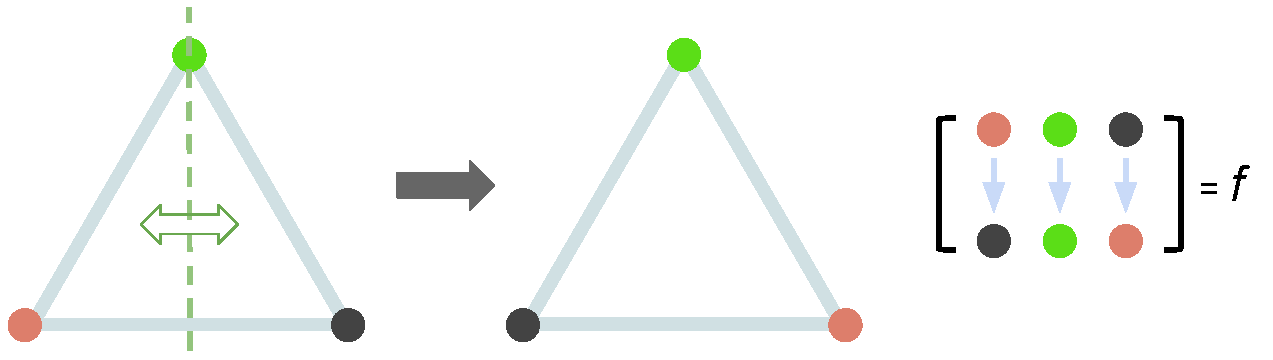
\includegraphics[width=0.8\paperwidth]{./images/Dihedral2.pdf}}
    \caption{The group action $f$ on dihedral group $D_3$ with order 6. $f$ is a horizontal flip.}
\end{figure}

We could said that the rotational symmetry group of an equilateral triangle, $C_3$, is isomorphic to
$\mathbb{Z}_3$. We can combine the horizontal reflection and rotations and form another reflection lines, 
which these reflection lines runs from one of the vertices to the center of the opposing side.

\begin{figure}[ht]
    \centering
    \makebox[\textwidth]{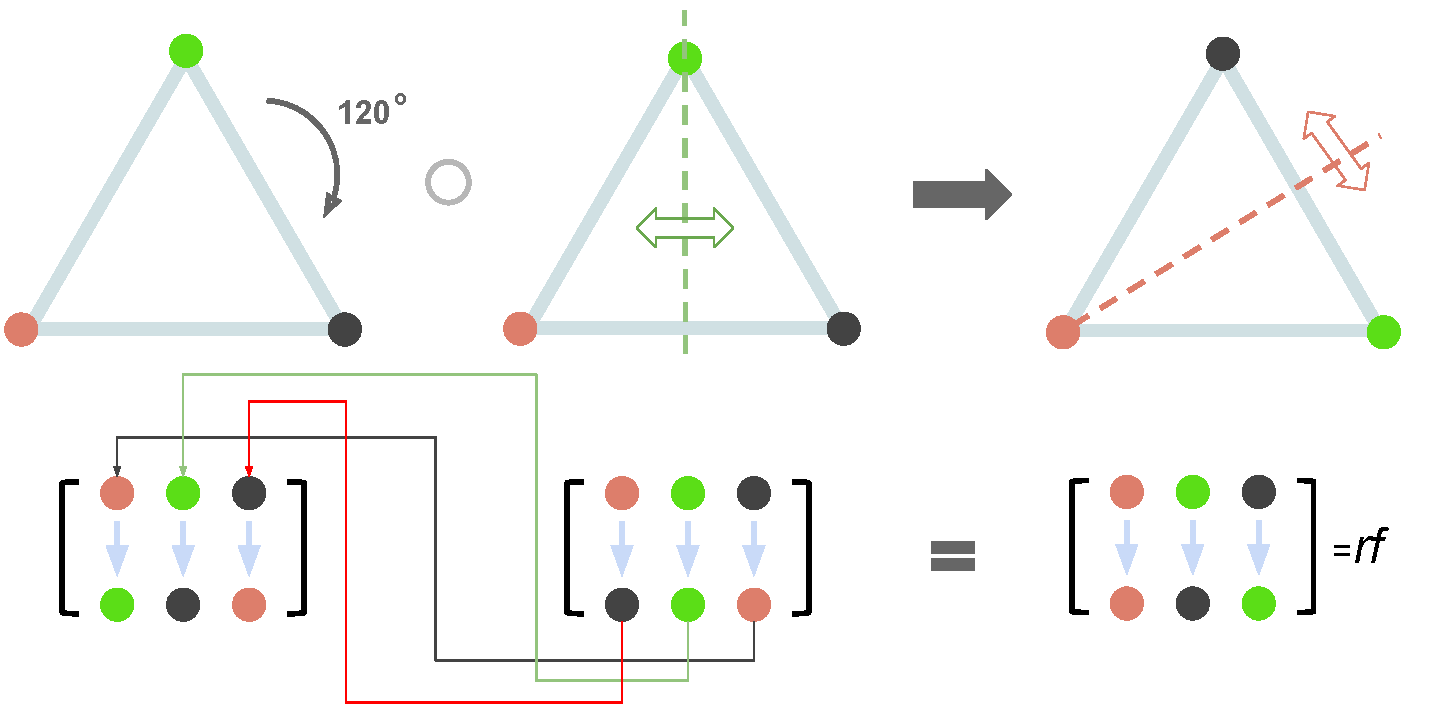
\includegraphics[width=0.8\paperwidth]{./images/Dihedral3.pdf}}
    \caption{The composition of $120\deg$ rotation with horizontal reflection form another reflection line at vertice}
\end{figure}

\begin{lemma}
    Dihedral group $D_3$ is isomorphic to $S_3$.
\end{lemma}

\section{Sylow's theorem}

\begin{theorem}
    $C_5 \times C_2$ and $C_{10}$ are two isomorphism classes.
\end{theorem}
\begin{proof}
    From the \textit{Third Sylow's theorem}, the number of Sylow 5-groups divides 2 and is $1 (mod 5)$, so there is only one Sylow 5-group.
    And there is a normal subgroup $K \trianglelefteq G$ such that $|K| = 5$.
\end{proof}

\section{Isomorphism}

\begin{example}
    The group $U(10)$ is not isomorphic to $U(12)$.
\end{example}

\begin{theorem}[Cayley's theorem]
    Every group is isomorphism to a group of permutation.
\end{theorem}

\section{Automorphisms}

\begin{definition}
    An isomorphism from a group $G$ onto itself is called an automorphism.
\end{definition}

\begin{example}
    Let the 2-dimensional cartesian plane
    \[
        \mathbb{R}^2 = \{ (a,b) | a, b \in \mathbb{R} \}.
    \]
    Then
    \[
        \phi(a,b) = (b,a)
    \]
    is an automorphism of the group $\mathbb{R}^2$ under componentwise addition.
\end{example}

\begin{example}
    Compute $\text{Aut}(\mathbb{Z}_{10})$.
\end{example}
\begin{solution}
    For any $\alpha \in \text{Aut}(\mathbb{Z}_{10})$ and for any $k \in \mathbb{Z}_{10}$. We define $k \mapsto k \alpha(1)$ such that 
    \[
        1 \mapsto \alpha_1 :\quad \mathbb{Z}_{10} \to \mathbb{Z}_{10}, \quad \alpha_1(x) = x
    \]
    \[
        3 \mapsto \alpha_3 :\quad \mathbb{Z}_{10} \to \mathbb{Z}_{10}, \quad \alpha_3(x) = 3x
    \]
    \[
        7 \mapsto \alpha_7 :\quad \mathbb{Z}_{10} \to \mathbb{Z}_{10}, \quad \alpha_7(x) = 7x
    \]
    \[
        9 \mapsto \alpha_9 :\quad \mathbb{Z}_{10} \to \mathbb{Z}_{10}, \quad \alpha_9(x) = 9x
    \]

    In fact, $\text{Aut}(\mathbb{Z}_{10})$ is isomorphic to $U(10) = \{ 1, 3, 7, 9\}$.
\end{solution}

\begin{definition}[Inner automorphisms]
    Let $G$ be a group, and let $a \in G$. The function $\phi_a$ defined by 
    \[
        \phi_a(x) = axa^{-1} \quad \text{for all } x \in G
    \]
    is called the inner automorphism of $G$ included by $a$.

    When $G$ is a group, we use $\text{Aut}(G)$ to denote the set of all automorphisms of $G$ and 
    $\text{Inn}(G)$ to denote the set of all inner automorphisms of $G$.
\end{definition}

\begin{theorem}
    The set of automorphisms of a group and the set of inner automorphisms of a group are both groups under the 
    operation of function composition.
\end{theorem}
\begin{proof}
    The set of inner automorphisms of $G$ included by $a$ is 
    \[
        \text{Inn}(G) = \{ \phi_a | \phi_a \text{ is an inner automorphism}  \}.
    \]
    Then satisfied the group properties:
    \begin{enumerate}
        \item We want to show $\forall \phi_a, \phi_b \in \text{Inn}(G), \quad \phi_a \circ \phi_b \in \text{Inn}(G)$.  

        Compute $(\phi_a \circ \phi_b)(g)$ for all $g$ in $G$,
        \begin{align*}
            (\phi_a \circ \phi_b)(g) &= \phi_a (\phi_b (g))\\
            &= \phi_a(bgb^{-1}) & \text{(Defn. of inner automorphism)}\\
            &= a(bgb^{-1})a^{-1}\\
            &= (ab)g(b^{-1}\, a^{-1})\\
            &= (ab)\, g\, (ab)^{-1} & \text{(Socks-shoes property)}\\
            &= \phi_{ab}(g) \in \text{Inn}(G)
        \end{align*}
        
        Thus $\text{Inn}(G)$ is closed under function composition.

        \item Next we want to show the associativity in $\text{Inn}(G)$, that is, 
        \[
            \forall \phi_a, \phi_b, \phi_c \in \text{Inn}(G), \quad \phi_a \circ (\phi_b \circ \phi_c) = (\phi_a \circ \phi_b) \circ \phi_c 
        \]

        we compute $\phi_a \circ (\phi_b \circ \phi_c)$.
        \begin{align*}
            [\phi_a \circ (\phi_b \circ \phi_c)](g) &= a(bc)g(bc)^{-1}a^{-1}\\
            &= (ab)c g \, c^{-1}\, b^{-1}\, a^{-1}\\
            &= {\color{cyan} (ab)}{\color{red} \underline{c\, g\, c^{-1}}}\, {\color{cyan} (ab)^{-1}}\\
            &= [{\color{cyan} (\phi_a \circ \phi_b)} \circ {\color{red} \underline{\phi_c}}](g)
        \end{align*}

        \item Suppose $e$ is the identity element of $G$, then $\phi_e(g) = ege^{-1} = g \in \text{Inn}(G)$. $\phi_e$ is the 
        identity of $\text{Inn}(G)$.

        \item For all $\phi_a \in \text{Inn}(G)$, there exists $\phi_{a^{-1}} \in \text{Inn}(G)$ such that 
        \begin{align*}
            \phi_a \circ \phi_{a^{-1}} &= a(a g^{-1} a^{-1})a^{-1}\\
            &= (a\,a^{-1}) g^{-1} (a\,a^{-1})\\
            &= g^{-1}
        \end{align*}
    \end{enumerate}

    We have shown that the inner automorphisms are group. Is $\text{Inn}(G)$ a subgroup of $\text{Aut}(G)$? Of course it is. We 
    are going to use one-step subgroup test to find out.

    \textbf{One-step subgroup test}:

    \begin{enumerate}
        \item First of all, we want to show 
        \[
            \forall \phi_a, \phi_b \in \text{Inn}(G), \phi_a \circ \phi_{b^{-1}} \in \text{Inn}(G).
        \]

        we compute
        \begin{align*}
            (\phi_a \circ \phi_{b^{-1}})(g) &= \phi_a (b g^{-1}b^{-1})\\
            &= a(b g^{-1}b^{-1})a^{-1}\\
            &= (ab)g^{-1}\,(ab)^{-1}\\
            &= \phi_{(ab)^{-1}} \in \text{Inn}(G)
        \end{align*}
    \end{enumerate}
\end{proof}

\section{Cosets}

\begin{example}
    Consider $G = \mathbb{Z}_9 = \{ 0, 1, 2, \ldots, 8 \} (\text{mod} \, 9)$. We take a cyclic subgroup 
    \[H = \langle 3 \rangle = \{0, 3, 6\}\] 
    which came from $(G, \oplus)$. All \textbf{left cosets} of $G$ with respect to $H$ are $\{ H, 1 \oplus H, 2 \oplus H \}$ where
    \begin{align*}
        &0 \oplus H = \{0 + 0, 0+ 3, 0 + 6\} (\text{mod} \, 9) = \{0, 3, 6\} = H\\
        &1H = 1 \oplus H = \{1 + 0, 1 + 3, 1 + 6\} (\text{mod} \, 9) = \{1, 4, 7\}\\
        &2H = 2 \oplus H = \{2 + 0, 2 + 3, 2 + 6\} (\text{mod} \, 9) = \{2, 5, 8\}\\
        &3H = 3 \oplus H = \{3 + 0, 3 + 3, 3 + 6\} (\text{mod} \, 9) = \{3, 6, 0\} = H
    \end{align*}

    As for the right cosets of $G$ with respect to $H$ are $\{ H, H \oplus 1, H \oplus 2 \}$. Pay attention that now the element of coset are being 
    added to right-hand side instead of from left side.

    \begin{align*}
        &0 \oplus H = \{0 + 0, 0+ 3, 0 + 6\} (\text{mod} \, 9) = \{0, 3, 6\} = H\\
        &H1 = H \oplus 1 = \{0 + 1, 3 + 1, 6 + 1\} (\text{mod} \, 9) = \{1, 4, 7\}\\
        &H2 = H \oplus 2 = \{0 + 2, 3 + 2, 6 + 2\} (\text{mod} \, 9) = \{2, 5, 8\}\\
        &H3 = H \oplus 3 = \{0 + 3, 3 + 3, 6 + 3\} (\text{mod} \, 9) = \{3, 6, 0\} = H
    \end{align*}
\end{example}

\section{Normal subgroups, Quotient groups}

\subsection{Normal subgroups}

\begin{definition}[Normal subgroups]
    A subgroup $H$ of $(G, \cdot)$ is called a normal subgroup if for all $g \in G$ we have 
    \begin{equation}
        gH = Hg.
    \end{equation}
    We shall denote that $H$ is a subgroup of $G$ by $H < G$, and that $H$ is a normal subgroup of $G$ 
    by $H \vartriangleleft G$. 
    
    If $H$ is a normal subgroup of $G$, and the order of $H$ is equal to the order of $G$, we called $H$ the proper normal subgroup, write as $H \trianglelefteq G$. 
\end{definition}

You should be very careful here. The equality $gH = Hg$ is a set equality. They are not constants or numbers! It says that a 
right coset is equal to left a coset, it is not an equality elementwise.

\begin{example}
    Let $\mathbb{R}[x]$ denote the group of all polynomial with real coefficients under normal addition. 

    For any $f$ in $\mathbb{R}[x]$, let $f'$ denote the derivative of $f$. Then the mapping $f \to f'$ is a homomorphism from 
    $\mathbb{R}[x]$ to itself. The kernel of the derivative mapping is the set of all constant polynomials $f(x) = c$.
\end{example}

Now suppose we have a group $(G, cdot)$, and $H$ is a normal subgroup of $G$, just said $H \vartriangleleft G$. The set $G/H$ is defined by 
\[
G/H = \{ gH \> | \> g \in H \}
\]



\begin{theorem}[Orbit-Stabilizer theorem]
    For any group action $\phi : G \to \text{Permutation}(S)$, and for any $s \in S$,
    \begin{equation}
        |\text{Orb}(s)| \cdot |\text{Stab}(s)| = |G|.
    \end{equation}
\end{theorem}

\newpage 
\begin{theorem}
    The group of rotations of a cube is isomorphic to $S_4$.
\end{theorem}
\begin{proof}
    We can proof it by visualizing the cube rigid motions.
    \begin{figure}[ht]
        \centering
        \begin{tikzpicture}
            \begin{scope}[scale=2,y={(0.2cm,0.3cm)},x={(1cm,0cm)}, z={(0cm,1cm)}]
                \coordinate (O) at (0, 0, 0);
            
                \draw[  very thick,Bcolor, dashed ] (0,0,1)--(0,0,-1);
                \draw[  very thick,Bcolor ] (0,0,-1.4)--(0,0,-1);
                \draw[  very thick,Bcolor ] (0,0,1.4)--(0,0,1);
            
                \draw[dotted, very thick,medgrey] (1,1,-1)--(-1,1,-1)--(-1,-1,-1);
                \draw[dotted, very thick,medgrey] (-1,1,-1)--(-1,1,1);
            
                \draw[thick,opacity=0.2,fill=Ccolor]  (1,1,1)--(1,-1,1)--(-1,-1,1)--(-1,1,1)--cycle; % top
                \draw[thick,opacity=0.2,fill=Ccolor] (1,-1,1)--(1,-1,-1)--(-1,-1,-1)--(-1,-1,1)--cycle; % front
                \draw[thick,opacity=0.2,fill=Acolor] (1,1,-1)--(1,1,1)--(1,-1,1)--(1,-1,-1)--cycle;
            
              \end{scope}
              \node[inner sep = 0cm,text width=\linewidth, align=center] at (0,-5.5)   () {One of three possible axes of rotation through the centers of opposite faces.\\ Each rotation could be $0^\circ$, $90^\circ$, $180^\circ$, or $270^\circ$, for a total of $3\cdot 4 = 12$ rotations of this type. But three in this count are the trivial identity rotation, which we only count once, so there are really 10 unique rotations along these axes. };
        \end{tikzpicture}
    \end{figure}

    \begin{figure}[ht]
        \centering
        \begin{tikzpicture}
            \begin{scope}[scale=2,y={(0.2cm,0.3cm)},x={(1cm,0cm)}, z={(0cm,1cm)}]
                \coordinate (O) at (0, 0, 0);
            
                \draw[  very thick,Bcolor, dashed ] (-1,1,1)--(1,-1,-1);
                \draw[  very thick,Bcolor ] (1.2,-1.2,-1.2)--(1,-1,-1);
                \draw[  very thick,Bcolor ] (-1.2,1.2,1.2)--(-1,1,1);
            
            
                \draw[  dotted, very thick,medgrey ] (1,1,-1)--(-1,1,-1)--(-1,-1,-1);
                \draw[dotted, very thick ,medgrey] (-1,1,-1)--(-1,1,1);
            
                \draw[thick,opacity=0.2,fill=Ccolor]  (1,1,1)--(1,-1,1)--(-1,-1,1)--(-1,1,1)--cycle; % top
                \draw[thick,opacity=0.2,fill=Ccolor] (1,-1,1)--(1,-1,-1)--(-1,-1,-1)--(-1,-1,1)--cycle; % front
                \draw[thick,opacity=0.2,fill=Acolor] (1,1,-1)--(1,1,1)--(1,-1,1)--(1,-1,-1)--cycle;
            
              \end{scope}
              \node[inner sep = 0cm,text width=\linewidth, align=center] at (0,-5.5)   () {One of four possible axes of rotation through opposite vertices. Each could be either $120^\circ$ or $240^\circ$, so there are $4 \cdot 2 = 8$ rotations of this type.};
        \end{tikzpicture}
    \end{figure}

    \newpage
    \begin{figure}[ht]
        \centering
        \begin{tikzpicture}
            \begin{scope}[scale=2,y={(0.2cm,0.3cm)},x={(1cm,0cm)}, z={(0cm,1cm)}]
                \coordinate (O) at (0, 0, 0);
            
                \draw[  very thick,Bcolor, dashed ] (0,1,1)--(0,-1,-1);
                \draw[  very thick,Bcolor ] (0,-1.2,-1.2)--(0,-1,-1);
                \draw[  very thick,Bcolor ] (0,1.2,1.2)--(0,1,1);
            
                \draw[  dotted, very thick,medgrey ] (1,1,-1)--(-1,1,-1)--(-1,-1,-1);
                \draw[dotted, very thick ,medgrey] (-1,1,-1)--(-1,1,1);
            
                  \draw[thick,opacity=0.2,fill=Ccolor]  (1,1,1)--(1,-1,1)--(-1,-1,1)--(-1,1,1)--cycle; % top
                  \draw[thick,opacity=0.2,fill=Ccolor] (1,-1,1)--(1,-1,-1)--(-1,-1,-1)--(-1,-1,1)--cycle; % front
                  \draw[thick,opacity=0.2,fill=Acolor] (1,1,-1)--(1,1,1)--(1,-1,1)--(1,-1,-1)--cycle;
            
              \end{scope}
              \node[inner sep = 0cm,text width=\linewidth, align=center] at (0,-4.5)   () {One of six possible axes of rotation through the centers of opposite edges. Only a $180^\circ$ rotation around these axes would preserve the shape, so we have only 6 rotations possible.};
        \end{tikzpicture}
    \end{figure}

    There are $10 + 8 + 6 = 24$ possible ways to rotate a cube, this is equal to the order of $S_4$. The order of $S_4$ is
    \[
        |S_4| = 4! = 4 \times 3 \times 2 \times 1 = 24.
    \]
\end{proof}

\section{Group homomorphisms}

\begin{definition}
    A group homomorphism is a map $f: (G,{\color{red} \diamond}_G) \to (H, {\color{cyan} \bullet}_H)$ that respects binary operations:
    \begin{equation}
        f(a) \> {\color{cyan} \bullet}_H \> f(b) = f(a \> {\color{red} \diamond}_G \> b) \quad \forall a, b \in G
    \end{equation}
\end{definition}

\section{Tutorials}

\begin{mdframed}
    \vspace{-0.25cm}
    \hspace{-0.25cm}
    \begin{Exercise}
        Prove whether the following group $G$ together with operation $*$ is a group.
        \begin{enumerate}
            \item Let $*$ defined on $G = \mathbb{R}$ by letting $a * b = ab \quad \forall a, b \in \mathbb{R}$.
            \item Let $*$ defined on $G = 2\mathbb{Z}$ by letting $a * b = a + b \quad \forall a, b \in 2\mathbb{Z}$.
            \item Let $*$ defined on $G = \mathbb{R}^\times$ by letting $a * b = \sqrt{ab} \quad \forall a, b \in \mathbb{R}^\times$.
            \item Let $*$ defined on $G = \mathbb{Z}$ by letting $a * b = \max \{a,b\} \quad \forall a, b \in \mathbb{Z}$.
        \end{enumerate}
    \end{Exercise}

    \vspace{0.752cm}
    \begin{Exercise}
        Determine whether the given set of matrices under the specified operation, matrix addition or multiplication, is a group.
        \begin{enumerate}
            \item All $2 \times 2$ diagonal matrices under matrix addition.
            \item All $2 \times 2$ diagonal matrices under matrix multiplication.
            \item All $2 \times 2$ diagonal matrices with no zero diagonal entry under under matrix multiplication.
            \item All $2 \times 2$ diagonal matrices with all diagonal entries either $1$ or $-1$ under matrix multiplication.
            \item All $2 \times 2$ upper-triangular matrices under matrix multiplication.
            \item All $2 \times 2$ upper-triangular matrices under matrix addition.
            \item All $2 \times 2$ upper-triangular matrices with determinant $1$ under matrix multiplication.
            \item All $2 \times 2$ upper-triangular matrices with determinant either $1$ or $-1$ under matrix multiplication.
        \end{enumerate}
    \end{Exercise}

    \vspace{0.752cm}
    \begin{Exercise}
        Prove whether 
        \[
            G = \biggl\{ \begin{bmatrix}
            a & b \\ c & d
            \end{bmatrix} \bigg \vert \> ad - bc \neq 0,\> a,b,c,d \in \mathbb{Z} \biggr\}
        \]
        is a group under matrix multiplication.
    \end{Exercise}

    \vspace{0.752cm}
    \begin{Exercise}
        Prove whether 
        \[
            G = \biggl\{ \begin{bmatrix}
            a & b \\ 0 & d
            \end{bmatrix} \bigg \vert \> ad \neq 0,\> a,b,d \in \mathbb{Z} \biggr\}
        \]
        is a non-abelian group under matrix multiplication.
    \end{Exercise}

    \vspace{0.752cm}
    \begin{Exercise}
        Prove whether 
        \[
            G = \biggl\{ \begin{bmatrix}
            a & b \\ 0 & a^{-1}
            \end{bmatrix} \bigg \vert \> a \neq 0,\> a,b \in \mathbb{Z} \biggr\}
        \]
        is an abelian group under matrix multiplication.
    \end{Exercise}

    \vspace{0.752cm}
    \begin{Exercise}
        Let $(G, *)$ be a group and suppose that 
        \[
            a * b * c = e \quad \forall a,b,c \in G.
        \]

        Show that $b * c * a = e$.
    \end{Exercise}

    \vspace{0.752cm}
    \begin{Exercise}
        Show that if every element of the group $G$ is its own inverse, then $G$ is abelian.
    \end{Exercise}

    \vspace{0.752cm}
    \begin{Exercise}
        Show that every group with identity $e$ and $x \cdot x = x$ for all $x \in G$ is abelian.
    \end{Exercise}

    \vspace{0.752cm}
    \begin{Exercise}
        Show that if $G$ is a finite group with identity $e$ and with even number of elements, then there is an 
        $a \neq e$ in $G$ such that $a * a = e$.
    \end{Exercise}

    \vspace{0.752cm}
    \begin{Exercise}
        Suppose $G$ is a group such that 
        \[
            (ab)^2 = a^2\, b^2 \quad \forall a, b \in G.
        \]

        Show that $G$ is abelian.
    \end{Exercise}

    \vspace{0.752cm}
    \begin{Exercise}
        Find the order of the following cyclic groups.
        \begin{enumerate}
            \item The subgroup of $U(6)$ generated by $\displaystyle \cos \biggl( \frac{2\pi}{3}\biggr) + i \sin \biggl( \frac{2\pi}{3}\biggr)$.
            \item The subgroup of $U(5)$ generated by $\displaystyle \cos \biggl( \frac{4\pi}{3}\biggr) + i \sin \biggl( \frac{4\pi}{3}\biggr)$.
            \item The subgroup of $\mathbb{Z}/4\mathbb{Z} \times \mathbb{Z}/6\mathbb{Z}$ generated by $(1,5)$.
        \end{enumerate}
    \end{Exercise}

    \vspace{0.752cm}
    \begin{Exercise}
        Let $a$ and $b$ be elements of a group $G$. Show that if $ab$ has finite order $n$, then $ba$ also has order $n$.
    \end{Exercise}

    \vspace{0.752cm}
    \begin{Exercise}
        Show that a group with no proper nontrivial subgroup is cyclic. 
    \end{Exercise}

    \vspace{0.752cm}
    \begin{Exercise}
        Let $G$ be a nonabelian group with center $Z(G).$ Show that there exists an abelian subgroup $H$ of 
        $G$ such that $Z(G) \subset H$ but $Z(G) \neq H$. 
    \end{Exercise}

    \vspace{0.752cm}
    \begin{Exercise}
        Find all subgroups of the following groups and draw the subgroups diagram for the subgroups. 
        Hence, list all orders of the subgroups of the given groups.
        \begin{enumerate}
            \item $\mathbf{Z}_{36}$
            \item $\mathbf{Z}_{60}$
        \end{enumerate} 
    \end{Exercise}

    \vspace{0.752cm}
    \begin{Exercise}
        \begin{enumerate}
            \item Find all the proper nontrivial subgroups of $\mathbb{Z}_2 \times \mathbb{Z}_2 \times \mathbb{Z}_2$.
            \item Find all the subgroups of $\mathbb{Z}_2 \times \mathbb{Z}_4$ of order 4. 
        \end{enumerate}
    \end{Exercise}

    \vspace{0.752cm}
    \begin{Exercise}
        \begin{enumerate}
            \item Are the groups $\mathbb{Z}_2 \times \mathbb{Z}_{12}$ and $\mathbb{Z}_4 \times \mathbb{Z}_{6}$ isomorphic?
            \item Are the groups $\mathbb{Z}_8 \times \mathbb{Z}_{10} \times \mathbb{Z}_{24}$ and $\mathbb{Z}_4 \times \mathbb{Z}_{12} \times \mathbb{Z}_{40}$ isomorphic?
        \end{enumerate}
    \end{Exercise}

    \vspace{0.752cm}
    \begin{Exercise}
        Find the conjugacy classes of dihedral group $D_8$. 
    \end{Exercise}

    \vspace{0.752cm}
    \begin{Exercise}
        Show that a group that has only finite number of subgroups must be a finite group.
    \end{Exercise}

    \vspace{0.752cm}
    \begin{Exercise}
        Find all cosets of the subgroup $4\mathbb{Z}$ of $\mathbb{Z}$.
    \end{Exercise}

    \vspace{0.752cm}
    \begin{Exercise}
        Compute the quotient group $\mathbb{Z}_{12}/ \langle 2 \rangle$.
    \end{Exercise}

    \vspace{0.752cm}
    \begin{Exercise}
        Show that if $H$ is a subgroup of index 2 in a finte group $G$, then every left coset of $H$ is also a 
        right coset of $H$.
    \end{Exercise}

    \vspace{0.752cm}
    \begin{Exercise}
        Let $\phi: G \to G$ be a mapping defined by 
                \[
                    \phi(x) = x^3 \quad \forall x \in G
                \]
                where $G = \mathbb{R} \setminus \{ 0 \}$ is a group defined under usual multiplication. Show that 
                $\phi$ is a homomorphism, and hence find $ker(\phi)$.
    \end{Exercise}

    \vspace{0.752cm}
    \begin{Exercise}
        Let $\phi: G \to G$ be a mapping defined by 
                \[
                    \phi(x) = 5^x \quad \forall x \in G
                \]
                where $G = \mathbb{R} \setminus \{ 0 \}$ is a group defined under usual multiplication. Show that 
                $\phi$ is a homomorphism, and hence find $ker(\phi)$.
    \end{Exercise}

    \vspace{0.752cm}
    \begin{Exercise}
        Let $\phi: G \to G$ be a mapping defined by 
                \[
                    \phi(x) = 7x \quad \forall x \in G
                \]
                where $G = \mathbb{Z}$ is a group defined under usual addition. Show that 
                $\phi$ is a homomorphism, and hence find $ker(\phi)$.
    \end{Exercise}

    \vspace{0.752cm}
    \begin{Exercise}
        Let $G$ be a group and $g$ an element in $G$. Consider the mapping $\phi:G \to G$ defined as 
        $\phi(x) = gxg^{-1}$. Show that $\phi$ is an isomorphism.
    \end{Exercise}

    \vspace{0.752cm}
    \begin{Exercise}
        Find $ker(\phi)$ for map $\phi : \mathbb{Z}_{10} \to \mathbb{Z}_{20}$ such that 
        $\phi(1) = 8$.
    \end{Exercise}

    \vspace{0.752cm}
    \begin{Exercise}
        Find $ker(\phi)$ for map $\phi : \mathbb{Z} \times \mathbb{Z} \to \mathbb{Z} \times \mathbb{Z}$ such that 
        $\phi(1,0) = (2, -3)$ and $\phi(0,1) = (-1, 5)$.
    \end{Exercise}

    \vspace{0.752cm}
    \begin{Exercise}
        Let $\phi: G \to H$ be a group homorphism. Show that $\phi(G)$ is abelian if and only if
        \[
            xyx^{-1}y^{-1} \in ker(\phi) \quad \forall x, y \in G.
        \]
    \end{Exercise}

    \vspace{0.752cm}
    \begin{Exercise}
        Consider $A$ the set of affine maps of $\mathbb{R}$, that is 
        \[
            A = \{ f : x \mapsto ax + b, a \in \mathbb{R}^*, b \in \mathbb{R} \}
        \]
        \begin{enumerate}
            \item Show that $A$ is a group with respect to the composition of map.
            \item Let 
                \[
                    N = \{ g: x \mapsto x + b, b \in \mathbb{R} \}
                \]

                Show that $N \vartriangleleft A$.
            \item Show that the quotient group $A/N$ is isomorphic to $\mathbb{R}^*$.
        \end{enumerate}
    \end{Exercise}

    \vspace{0.752cm}
    \begin{Exercise}
        Let $G = S_4$ and let 
        \[
            H = \{ e, (1\> 2)(3 \> 4), (1\> 3)(2\> 4), (1\> 4)(2 \> 3)\}
        \]
        \begin{enumerate}
            \item Show that $H$ is a normal subgroup of $G$.
            \item Let $\overline{H} = \{ \sigma \in S_4 \> | \> \sigma(4) = 4 \}$. Define $\sigma : \overline{H} \to \text{Aut}(H)$
                by $\sigma(\tau) = \sigma \tau \sigma^{-1}$ for $\sigma \in \overline{H}$. Prove that 
                \[
                    \overline{H} \ltimes_\sigma H \cong S_4.
                \]
        \end{enumerate}
    \end{Exercise}

    \vspace{0.752cm}
    \begin{Exercise}
        Find (up to isomorphism) all abelian groups of order 45.
    \end{Exercise}

    \vspace{0.752cm}
    \begin{Exercise}
        Show that any group of order $p^2$ is abelian.
    \end{Exercise}

    \vspace{0.752cm}
    \begin{Exercise}
        Let $G$ be a group of order $pq$, where $p$ and $q$ are prime numbers. Show that every proper subgroup of $G$
        is cyclic.
    \end{Exercise}


    \vspace{0.752cm}
    \begin{Exercise}
        If $H, K \leq G$, show that $H \cap K \leq G$.
    \end{Exercise}

    \vspace{0.752cm}
    \begin{Exercise}
        If $N \vartriangleleft G$ and $H \leq G$, show that $NH \leq G$.
    \end{Exercise}

    \vspace{0.752cm}
    \begin{Exercise}
        If $N_1, N_2 \vartriangleleft G$, show that $N_1 \cap N_2 \vartriangleleft G$.
    \end{Exercise}


    \vspace{0.752cm}
    \begin{Exercise}
        If $N \vartriangleleft G$ and $H \leq G$, show that $H \cap N \vartriangleleft G$.
    \end{Exercise}
\end{mdframed}